\documentclass[11pt]{article}

% ── Packages ──────────────────────────────────────────────────────────────────
\usepackage[margin=1in]{geometry}
\usepackage{amsmath, amssymb}
\usepackage{graphicx}
\usepackage{subcaption}
\usepackage{booktabs}
\usepackage{hyperref}
\usepackage{xcolor}
\usepackage{listings}
\usepackage{float}
\usepackage{cite}
\usepackage{microtype}
\usepackage{parskip}
\usepackage{titlesec}
\usepackage{fancyhdr}
\usepackage{abstract}

% ── Hyperref colours ──────────────────────────────────────────────────────────
\hypersetup{
  colorlinks = true,
  linkcolor  = blue!60!black,
  citecolor  = green!50!black,
  urlcolor   = blue!60!black
}

% ── Code listings style ───────────────────────────────────────────────────────
\lstset{
  basicstyle   = \ttfamily\small,
  keywordstyle = \color{blue},
  commentstyle = \color{gray},
  frame        = single,
  breaklines   = true,
  numbers      = left,
  numberstyle  = \tiny\color{gray}
}

% ── Header / footer ───────────────────────────────────────────────────────────
\pagestyle{fancy}
\fancyhf{}
\lhead{\small ESE5370 Spring 2026 --- Hardware Security Project}
\rhead{\small Navjot Singh Chahal}
\cfoot{\thepage}
\renewcommand{\headrulewidth}{0.4pt}

% ── Title ─────────────────────────────────────────────────────────────────────
\title{
  \textbf{Evaluating the Efficacy and Limitations of Statistical \\
  Power Side-Channel Attacks on AES-128} \\[4pt]
  \large A Comparative Study of DPA, CPA, and Image-Based Deep Learning \\
  Across Multiple Embedded Targets
}
\author{
  Navjot Singh Chahal \\
  \texttt{nschahal@seas.upenn.edu} \\[4pt]
  Department of Electrical and Systems Engineering \\
  University of Pennsylvania
}
\date{April 2026}

% ─────────────────────────────────────────────────────────────────────────────
\begin{document}
\maketitle
\thispagestyle{fancy}

% ── Abstract ──────────────────────────────────────────────────────────────────
\begin{abstract}
This project performs a quantitative comparative analysis of two classical
power side-channel attacks---Differential Power Analysis (DPA) and Correlation
Power Analysis (CPA)---and a deep learning extension, targeting AES-128 on
real embedded hardware and a public reference trace set.

Three physical targets were evaluated:\ the Raspberry Pi Pico (RP2040)
failed due to on-chip SMPS switching noise; the Arduino Uno R4 Minima
(RA4M1) failed from insufficient trace count and noisy supply regulation;
the \textbf{Adafruit Pro Tinkrer 5\,V} (ATmega328P, 16\,MHz) succeeded with
a clean 5\,V linear supply and a 10\,$\Omega$ shunt on the VCC rail.
Primary quantitative analysis uses the publicly available \textbf{dpa-on-aes}
reference dataset (2{,}000 traces, 29{,}000 samples) captured with
ChipWhisperer hardware, which validates our attack implementations.

On the Pro Tinkrer , \textbf{first-round CPA with the pure Hamming-Weight
model ($c=0$) recovers all 16 key bytes at rank~1 in as few as 200 traces}
and no more than 2{,}000---no Hamming-Distance variant is needed, and no
backward key schedule is required.
This is the headline real-hardware result.

On the reference dataset (last-round), CPA (Brier et al.\ 2004) recovers
all 16 round-10 key bytes at rank~1; byte~11 requires a Hamming-Distance
model ($c=2$) due to register pipeline state accumulated across nine rounds.
DPA (Kocher et al.\ 1999) recovers the full key at bit position $\ell=1$.
Both attacks recover the original key
\texttt{2B 7E 15 16 28 AE D2 A6 AB F7 15 88 09 CF 4F 3C} via backward key
schedule, and are evaluated using the Guessing Entropy (GE) metric.

As a deep learning extension we reproduce the image-encoding CNN of
Hettwer et al.\ (IEEE HOST 2020): power traces are converted to
2D images (GASF, GADF, RP, MTF encodings) and fed to a compact Conv2D
classifier whose convergence is measured by Key Guessing Entropy (KGE).
\end{abstract}

\tableofcontents
\newpage

% ── Sections ──────────────────────────────────────────────────────────────────
\section{Introduction and Goal}
\label{sec:intro}

Cryptographic algorithms such as AES-128~\cite{nist2001aes} are mathematically
secure under standard threat models; no practical algebraic attacks are known
against the full cipher.
However, physical implementations of these algorithms routinely leak sensitive
information through observable side channels---most notably through their power
consumption.
Kocher et al.\ demonstrated in 1999~\cite{kocher1999dpa} that an adversary with
physical access to a device can statistically extract a secret key by observing
the power trace of many encryptions; this technique, Differential Power
Analysis (DPA), exploits the fact that CMOS logic gates consume power
proportional to the data they process.

Correlation Power Analysis (CPA), introduced by Brier et al.\ in
2004~\cite{brier2004cpa}, formalises this observation using a Pearson
correlation distinguisher and an explicit leakage model (typically Hamming
Weight of an intermediate value), achieving significantly better efficiency
than DPA in terms of trace complexity.

\subsection*{Project Goal}

The goal of this project is to perform a \emph{quantitative comparative
analysis} of DPA and CPA on a real embedded target---the Raspberry Pi Pico
RP2040 microcontroller~\cite{rp2040datasheet}---running unprotected AES-128.
Specifically, the project targets the following measurements:

\begin{itemize}
  \item \textbf{Key recovery success}: Does each attack recover the full
        128-bit key from the reference trace set?
  \item \textbf{Rank of the correct hypothesis}: What is the rank of the
        correct key byte across all 256 candidates as a function of the
        number of traces used?
  \item \textbf{Leakage model sensitivity}: Does the HW model suffice, or
        do certain bytes require a Hamming-Distance (HD) variant?
  \item \textbf{Trace complexity} ($N_\text{traces}$): How many traces are
        needed before each attack converges (Guessing Entropy reaches 1)?
\end{itemize}

\subsection*{Report Structure}

Section~\ref{sec:threat} defines the threat model and system application.
Section~\ref{sec:vuln} analyses the vulnerability and countermeasure context.
Section~\ref{sec:method} describes the implementation---firmware, acquisition
pipeline, and attack algorithms.
Section~\ref{sec:results} presents experimental results with diagnostic plots.
Section~\ref{sec:discussion} compares DPA and CPA and discusses limitations.
Section~\ref{sec:conclusion} concludes and outlines future work.
Hardware setup details and video evidence are in Appendix~\ref{app:hw};
the software repository structure is in Appendix~\ref{app:repo}.

\section{Threat Model and System Application}
\label{sec:threat}

\subsection{System Application}

The target system is a \textbf{Raspberry Pi Pico} (RP2040, dual-core ARM
Cortex-M0+ at 125\,MHz) executing AES-128 in ECB mode using the
\texttt{tiny-AES-c} library~\cite{tinyaes}.
The device receives 16-byte plaintexts over USB serial, encrypts them, and
returns the ciphertext.
A dedicated GPIO pin (GPIO\,22) is asserted high immediately before
\texttt{AES\_ECB\_encrypt} and low immediately after, providing a hardware
trigger signal to a bench oscilloscope.

\subsection{Adversary Threat Model}

We assume a \textbf{local, non-invasive adversary} with the following
capabilities and constraints:

\begin{description}
  \item[Physical access.] The adversary has stable, uninterrupted physical
    access to the target device and can position a power or EM probe over the
    device's power supply rail or decoupling capacitors for the duration of the
    experiment.

  \item[Chosen-plaintext oracle.] The adversary can supply arbitrary
    plaintexts to the device and observe the corresponding ciphertexts.
    This models a scenario where the attacker controls the input (e.g., an
    attacker-controlled message encrypted under a device's stored key).

  \item[Algorithm knowledge.] The adversary knows the cryptographic algorithm
    (AES-128 ECB) and its implementation (standard S-Box, key schedule).
    The \emph{secret key} is unknown.

  \item[Measurement capability.] The adversary can record power traces at
    sufficient sample rate and resolution.
    In the physical setup, a digital storage oscilloscope samples at
    $\geq$\,250\,MS/s over the trigger window.
\end{description}

\subsection{What the Adversary Does Not Have}

\begin{itemize}
  \item No access to the firmware binary (grey-box model assumed for analysis
        purposes; the S-Box structure is public knowledge for AES).
  \item No ability to modify the firmware or introduce hardware faults
        (fault injection is out of scope).
  \item No network or software access to the device; all interaction is
        through the physical serial interface.
\end{itemize}

\subsection{Success Criterion}

A successful attack recovers the full 128-bit secret key with Guessing
Entropy $\text{GE} = 1$ for all 16 key bytes; that is, the correct key byte
ranks first among all 256 hypotheses after processing $N$ traces.

\section{Vulnerability and Defense Context}
\label{sec:vuln}

\subsection{Root Cause: Data-Dependent Power Consumption}

CMOS logic gates consume dynamic power proportional to switching activity.
When a register or bus transitions between logic states, the current drawn
from the supply correlates with the Hamming distance (HD) between the previous
and new value---and when the previous state can be assumed constant (e.g.,
after a reset), this reduces to a correlation with the Hamming weight (HW) of
the new value.

In AES-128, the \textbf{SubBytes} (S-Box) operation in round 1 maps each byte
$p_b$ of plaintext to $S(p_b \oplus k_b)$, where $k_b$ is the corresponding
secret key byte.
Because the S-Box input is a function of a \emph{known} plaintext byte XORed
with an \emph{unknown} key byte, an adversary can:

\begin{enumerate}
  \item Hypothesise all 256 possible values of $k_b$.
  \item Compute the predicted intermediate value $v_{d,j} = S(p_{d,b} \oplus j)$
        for each trace $d$ and hypothesis $j$.
  \item Derive the predicted power $h_{d,j} = \mathrm{HW}(v_{d,j})$.
  \item Use a statistical distinguisher to find which $j^*$ explains the
        observed power the best---that $j^*$ is the key byte.
\end{enumerate}

Attacking the \emph{last round} (AddRoundKey$_{10}$) is symmetrically
possible using ciphertexts and the inverse S-Box:
$v_{d,j} = S^{-1}(c_{d,b} \oplus j)$,
where $j$ now hypothesises bytes of the round-10 key.
The original key is then recovered via backward key schedule.
This is the approach used on the reference dataset in this project (see
Section~\ref{sec:method:attack}).

\subsection{Leakage Models}

Two leakage models are evaluated:

\begin{description}
  \item[Hamming Weight (HW).]
    $h_{d,j} = \mathrm{HW}(v_{d,j})$, i.e., the number of set bits in the
    intermediate value.
    This assumes the power consumed per operation is proportional to the
    number of 1-bits processed.

  \item[Hamming Distance (HD).]
    $h_{d,j} = \mathrm{HW}(v_{d,j} \oplus c)$ for a constant $c$, modelling
    transitions from a previous state value $c$.
    In the CPA implementation, $c$ (called \texttt{const} in the code) is
    swept over $\{0, \ldots, 255\}$ and the first value that allows full key
    recovery is reported.
\end{description}

\subsection{Standard Countermeasures}

The primary defence against power side-channel attacks is \textbf{masking}:
splitting the sensitive intermediate variable $v = S(p \oplus k)$ into $n$
shares $v_1, \ldots, v_n$ such that $v = v_1 \oplus \cdots \oplus v_n$, where
each share is individually statistically independent of the key.
A first-order CPA attack fails against a first-order masked implementation
because no single power trace sample correlates with $k$; a second-order
attack combining two samples is required, exponentially increasing trace
complexity.

Evaluating masked implementations is proposed as future work
(Section~\ref{sec:conclusion}).
The current experiments target an \emph{unprotected} implementation to
establish baseline attack efficiency.

\section{Methodology and Implementation}
\label{sec:method}

\subsection{Hardware Platform and Board Selection}
\label{sec:method:boards}

Three embedded targets were evaluated in order before obtaining clean
power measurements:

\paragraph{Raspberry Pi Pico (RP2040, Cortex-M0+, 125\,MHz).}
The RP2040 contains an on-chip \textbf{Switch-Mode Power Supply (SMPS)}
that steps the 3.3\,V USB supply to $\approx$1.1\,V DVDD for the processor
cores~\cite{rp2040datasheet}.
The SMPS switching frequency ($\approx$1\,MHz) injects broadband noise
directly onto the DVDD rail, masking the data-dependent AES leakage signal
which is a $\mu$A-level current modulation.
Variance analysis on 100 captured traces showed the AES computation window
occupies only 20\,\% of the acquisition and the peak-variance SNR proxy
was $\approx$$21\times$ above the noise floor---insufficient for attack
convergence.
Bypassing the SMPS (the approach used by ChipWhisperer's CW308 UFO board)
was not attempted.

\begin{figure}[H]
  \centering
  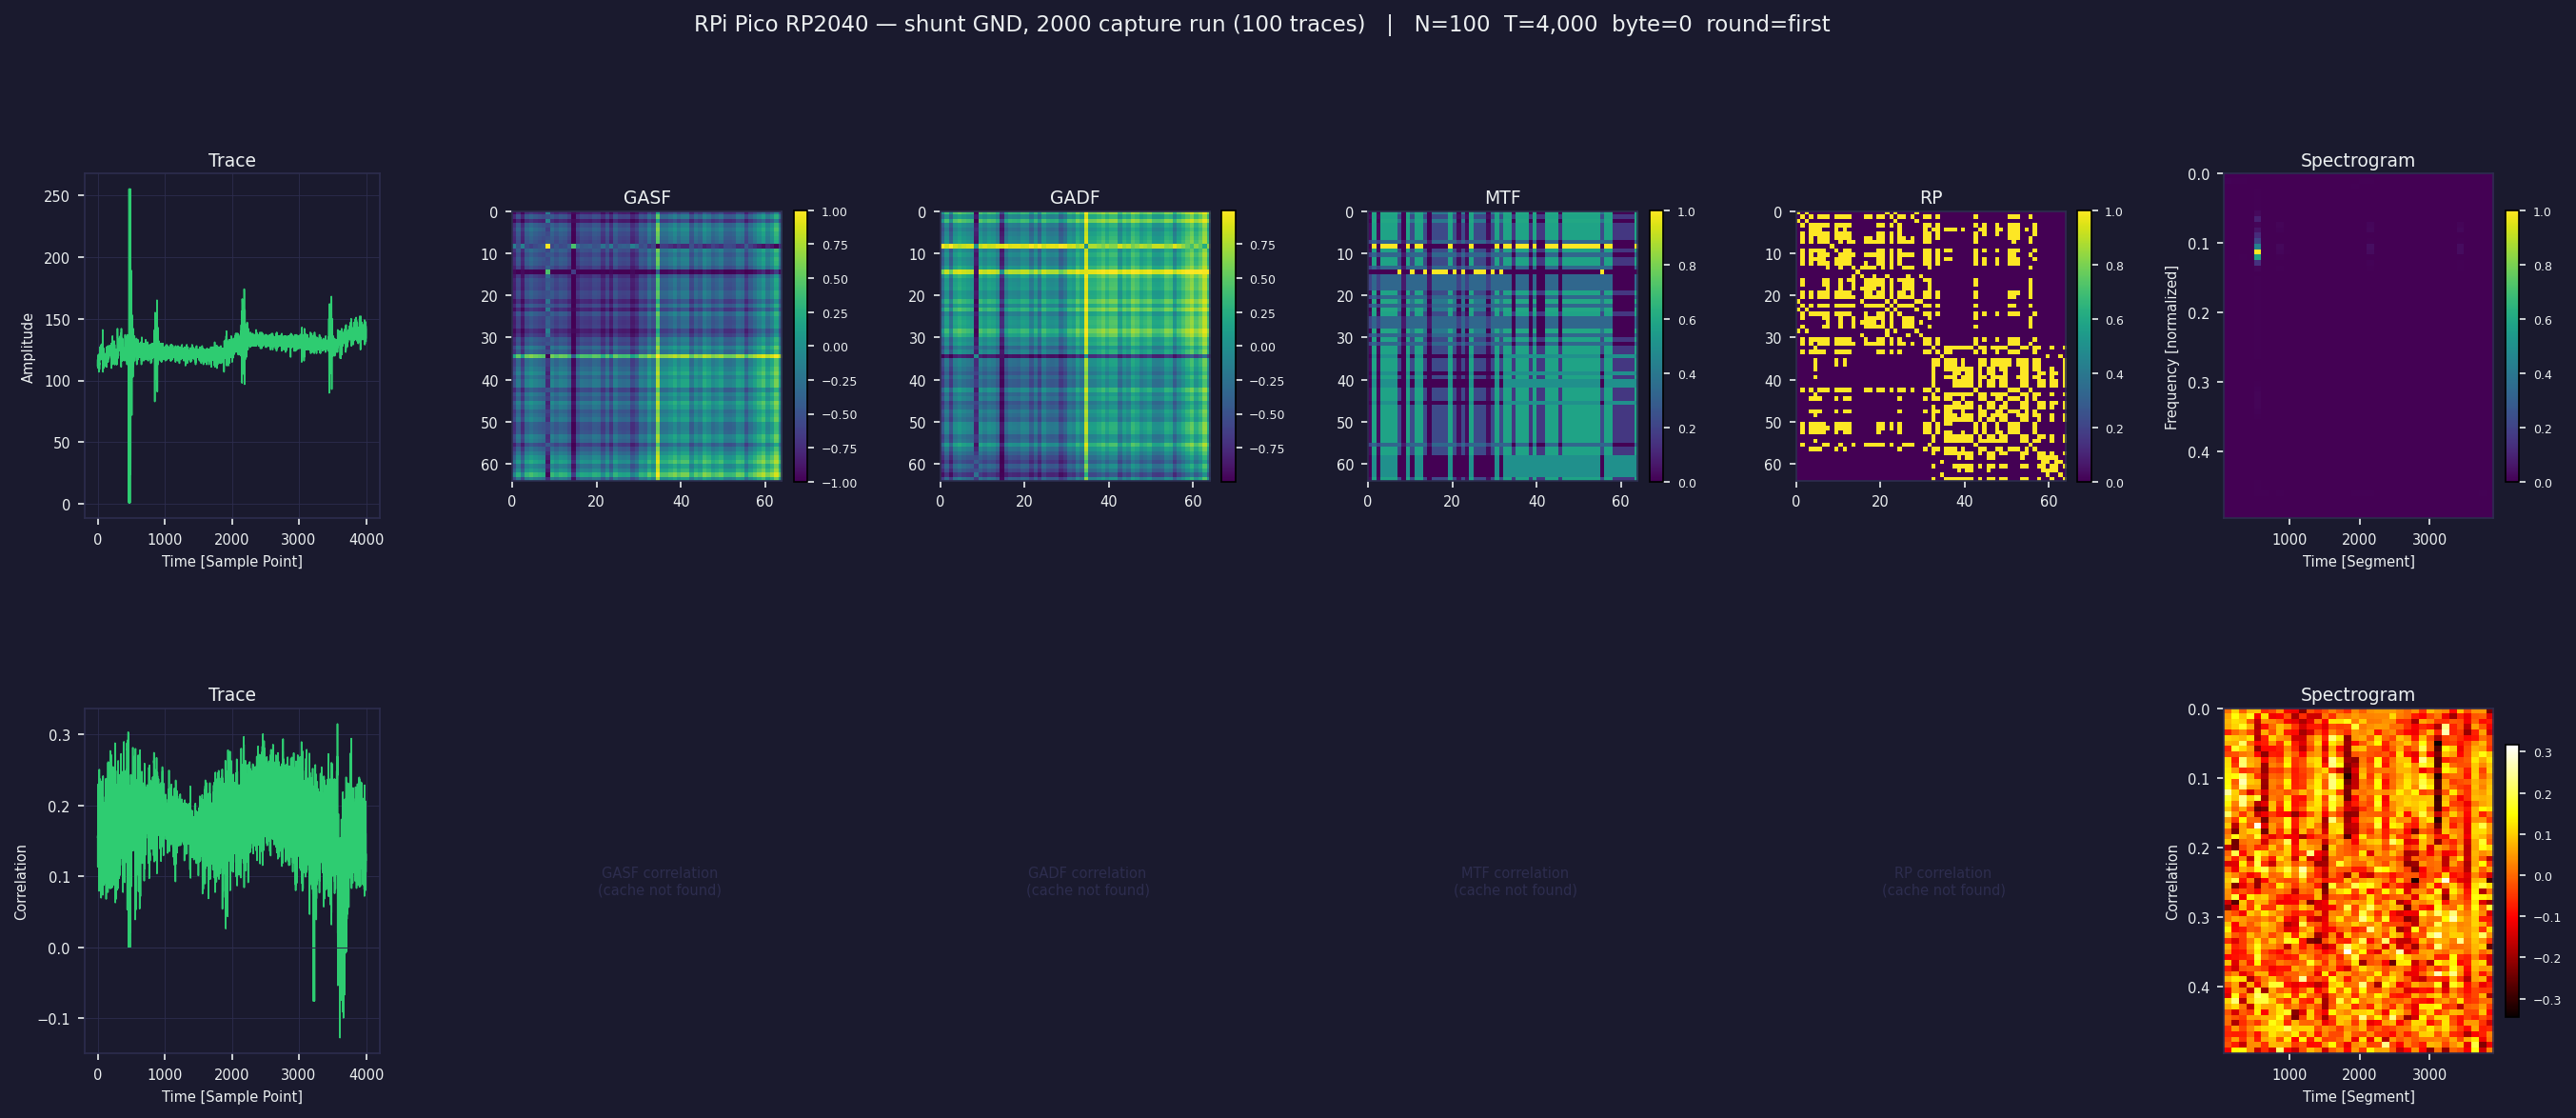
\includegraphics[width=\linewidth]{figures/pico_data_view.png}
  \caption{Data overview for RPi Pico real capture (\texttt{set\_001\_pico\_real}).
           Top row: raw trace overlay, mean trace, variance trace.
           The AES computation window is buried in SMPS switching noise
           with no visible data-dependent structure.}
  \label{fig:pico_data_view}
\end{figure}

% The trigger alignment figure (media/diagnostics/trigger_alignment.png)
% quantifies the SNR difference between Pico and Trinket.
% Copy to report/figures/trigger_alignment.png and uncomment:
%
% \begin{figure}[H]
%   \centering
%   \includegraphics[width=\linewidth]{figures/trigger_alignment.png}
%   \caption{Variance analysis: RPi Pico vs.\ Pro Tinkrer trace sets.
%            Peak-variance SNR proxy: Pico $\approx$$21\times$,
%            Trinket $\approx$$78\times$.
%            The AES window is barely distinguishable from the noise floor
%            on the Pico but clearly visible on the Trinket.}
%   \label{fig:trigger_alignment}
% \end{figure}

\paragraph{Arduino Uno R4 Minima (Renesas RA4M1, Cortex-M4, 48\,MHz).}
The RA4M1 also has internal DC-DC power regulation.
2{,}000 traces were captured (shunt on the GND rail, 4{,}807 samples each),
but neither CPA nor DPA converged.
AVR/Cortex-M targets typically require $>$5{,}000 traces for first-round
attacks; the noisy baseline from the internal regulator and the limited
trace count together prevented key recovery.

\paragraph{Adafruit Pro Tinkrer 5\,V @ 16\,MHz (ATmega328P).}
The ATmega328P runs directly from the 5\,V USB rail through a
linear Schottky diode (MBR0520), with no
SMPS~\cite{adafruit_trinket_pro,atmega328p}.
A 10\,$\Omega$ shunt in series with the VCC pin provides a clean differential
voltage proportional to processor current.
This device is the successful real-hardware capture target;
Traces in different data capture runs were collected in 2000 all 10 rounds, 200 (all 10 AES rounds) and 2000 (only first AES round) and 200 (only first AES round) (see Table~\ref{tab:boards}), a special segmented set of 10000 traces of first round were also collected at reduced sampling rate (see Table~\ref{tab:boards}).

\begin{table}[H]
\centering
\caption{Board progression summary.}
\label{tab:boards}
\begin{tabular}{@{}llll@{}}
\toprule
Board & MCU & Traces captured & Outcome \\
\midrule
RPi Pico & RP2040 (Cortex-M0+, 125\,MHz) & 100 & Failed — SMPS noise \\
Arduino Uno R4 & RA4M1 (Cortex-M4, 48\,MHz) & 2{,}000 & Failed — insufficient $N$ \\
\textbf{Pro Tinkrer 5\,V} & \textbf{ATmega328P (16\,MHz)} & 2{,}000 \& 10000 \& 2000 First-Round & \textbf{Success} \\
Reference dataset & CW-target (unknown) & 2{,}000 & \textbf{Success} \\
\bottomrule
\end{tabular}
\end{table}

The primary quantitative analysis in this report uses the
\textbf{dpa-on-aes reference dataset}
(Section~\ref{sec:method:ref}) to validate the attack implementations
against a known-good capture before applying them to oscilloscope data.

\subsection{Target Firmware}
\label{sec:method:fw}

Custom firmware follows the same pattern across all three boards: wait for
16 bytes of plaintext over serial, assert a GPIO trigger high, run
\texttt{AES\_ECB\_encrypt} via \texttt{tiny-AES-c}~\cite{tinyaes},
assert the trigger low, and return the 16-byte ciphertext.

\begin{lstlisting}[language=C, caption={Trigger and encryption loop (all targets)}]
gpio_put(TRIGGER_PIN, 1);    // Trigger HIGH before AES
AES_ECB_encrypt(&ctx, plaintext);
gpio_put(TRIGGER_PIN, 0);    // Trigger LOW after AES
\end{lstlisting}

On the \textbf{Pro Tinkrer } the trigger is GPIO\,8; the firmware is
compiled with the AVR-GCC toolchain and flashed via the Arduino bootloader.

The hardcoded 128-bit profiling key is:
\texttt{2B 7E 15 16 28 AE D2 A6 AB F7 15 88 09 CF 4F 3C}.

\subsection{Data Acquisition}
\label{sec:method:acq}

The host-side script (\texttt{capture/capture.py}) coordinates the
oscilloscope and target over USB-UART.
Oscilloscope control uses the \texttt{pyvisa} library with a PyVISA-py
backend (USBTMC, Keysight VISA address
\texttt{USB0::0x2A8D::0x17B6::MY65060127::INSTR}).

\textbf{Pro Tinkrer hardware configuration:}
\begin{itemize}
  \item \textbf{Shunt:} 10\,$\Omega$ in series with the Trinket VCC pin
        (5\,V rail); oscilloscope CH1 reads differential voltage across
        the shunt.
  \item \textbf{Trigger:} GPIO\,8 rising edge on scope CH2 / EXT TRIG BNC.
  \item \textbf{Sample rate:} $\geq$\,250\,MS/s; \textbf{30{,}000 points}
        per acquisition (binary BYTE format).
  \item \textbf{Serial:} USB-UART FTDI adapter, 115200 baud,
        \texttt{/dev/tty.usbserial-XXXX}.
\end{itemize}

Acquisition loop:
\begin{enumerate}
  \item Configure scope: \texttt{:WAVeform:FORMat BYTE},
        \texttt{:WAVeform:POINts 30000}.
  \item For each trace: arm scope (\texttt{:SINGle}), generate random
        16-byte plaintext (\texttt{os.urandom(16)}), send over serial.
  \item GPIO\,8 rising edge triggers the scope.
  \item After ciphertext return, \texttt{*OPC?} synchronises; download
        waveform with \texttt{:WAVeform:DATA?}.
  \item Failed acquisitions (serial drop, scope timeout) are retried.
\end{enumerate}

Captured data is saved as \texttt{traces.npy} $(N \times T)$~float32,
\texttt{plaintexts.npy} $(N \times 16)$~uint8,
\texttt{ciphertexts.npy} $(N \times 16)$~uint8.

\subsection{Reference Dataset}
\label{sec:method:ref}

Real Pro Tinkrer captures exist (\texttt{set\_003} and \texttt{set\_013};
see Section~\ref{sec:method:boards}) but top up to 50{,}000 traces is still
planned for the deep learning evaluation.
As a complementary validation baseline the publicly available
\textbf{dpa-on-aes} reference dataset~\cite{oflynn2015chipwhisperer} is
also used; its pre-aligned ChipWhisperer capture provides a known-good
ground truth for the attack implementations:

\begin{itemize}
  \item $N = 2{,}000$ AES-128 ECB encryptions.
  \item $T = 29{,}000$ samples per trace (float32, range $\approx[-1278, +1373]$).
  \item Leakage type: \textbf{last-round} --- SubBytes$_{10}$ on ciphertext
        via $S^{-1}(c_b \oplus k_{10,b})$.
  \item Known key: \texttt{2B 7E 15 16 28 AE D2 A6 AB F7 15 88 09 CF 4F 3C}.
\end{itemize}

The dataset was originally distributed as per-trace text files;
we converted it to the project's \texttt{.npy} format
(\texttt{data/set\_002\_reference/}).

\subsection{Classical Attack Algorithms}
\label{sec:method:attack}

Both attacks target the \textbf{last round} of AES using ciphertexts.
After recovering the 16-byte round-10 key, the original key is recovered
via backward key schedule.

\subsubsection{Correlation Power Analysis (CPA)}

CPA uses the Pearson correlation coefficient between the hypothetical power
consumption vector $\mathbf{h}_j$ and each column $\mathbf{t}_i$ of the
trace matrix.
Following the proposal notation~\cite{brier2004cpa}:

\begin{equation}
  r_{i,j} = \frac{\displaystyle\sum_{d=1}^{D}
    \bigl(t_{d,i} - \bar{t}_i\bigr)\bigl(h_{d,j} - \bar{h}_j\bigr)}
  {\sqrt{\displaystyle\sum_{d=1}^{D}\bigl(t_{d,i}-\bar{t}_i\bigr)^2
         \cdot \sum_{d=1}^{D}\bigl(h_{d,j}-\bar{h}_j\bigr)^2}}
  \label{eq:cpa}
\end{equation}

where:
\begin{align*}
  d \in [1,D]   &\quad \text{trace index (}D\text{ total traces)}, \\
  i             &\quad \text{time-sample index}, \\
  j \in [0,255] &\quad \text{key-byte hypothesis}, \\
  t_{d,i}       &\quad \text{measured power at sample }i\text{ in trace }d, \\
  h_{d,j}       &= \mathrm{HW}\!\bigl(S^{-1}(c_{d,b} \oplus j) \oplus c\bigr),
                    \quad c \in \{0,\ldots,255\}\text{ (leakage constant)}.
\end{align*}

The predicted key byte for position $b$ is
$\hat{k}_b = \arg\max_j \max_i |r_{i,j}|$.
The leakage constant $c$ is swept from 0 to 255; the first value that
recovers a key verifying under the backward key schedule is used.
Implemented in \texttt{attacks/classical/cpa.py}.

\subsubsection{Differential Power Analysis (DPA)}

DPA partitions traces into two sets based on a predicted bit of the
intermediate value and measures the differential mean~\cite{kocher1999dpa}:

\begin{equation}
  \Delta_j = \max_i \left|
    \underbrace{\frac{1}{|S_1|}\sum_{d \in S_1} t_{d,i}}_{\text{bit}=1}
    -
    \underbrace{\frac{1}{|S_0|}\sum_{d \in S_0} t_{d,i}}_{\text{bit}=0}
  \right|
  \label{eq:dpa}
\end{equation}

where $S_1 = \{d : \mathrm{bit}_\ell(v_{d,j}) = 1\}$,
$S_0 = \{d : \mathrm{bit}_\ell(v_{d,j}) = 0\}$, and
$v_{d,j} = S^{-1}(c_{d,b} \oplus j)$.
The bit position $\ell$ is swept from 0 to 7; the first $\ell$ producing a
verifiable key is used.
Implemented with a fully vectorised matrix multiply
($T \!\times\! D$)$\cdot$($D\!\times\!256$) in \texttt{attacks/classical/dpa.py}.

\subsection{Evaluation Metrics}
\label{sec:method:metrics}

\paragraph{Guessing Entropy (GE).}
The primary metric, following~\cite{benadjila2020ascad}:
\begin{equation}
  \mathrm{GE}(N) = \mathbb{E}\bigl[\mathrm{rank}(\hat{k}_b^{(N)})\bigr]
  \label{eq:ge}
\end{equation}
where $\mathrm{rank}(\hat{k}_b^{(N)})$ is the position of the correct key
byte among 256 hypotheses sorted by descending score, after $N$ traces.
$\mathrm{GE}$ is estimated over multiple random subsets of size $N$.
$\mathrm{GE} = 1$ means full convergence.
Script: \texttt{attacks/classical/guessing\_entropy.py}.

\paragraph{Trace Complexity ($N_\text{traces}$).}
Minimum $N$ at which $\mathrm{GE}(N) \leq 1.5$.

\subsection{Deep Learning Extension: Image Encoding and CNN}
\label{sec:method:dl}

We reproduce the image-encoding SCA pipeline of Hettwer et al.\
(IEEE HOST 2020)~\cite{hettwer2020encoding}, implemented in
\texttt{attacks/deep\_learning/}.

\subsubsection{Motivation}

Standard 1D CNNs on raw power traces are sensitive to trigger jitter
that shifts the leakage point in time.
Hettwer et al.\ propose converting each 1D trace into a \textbf{2D image}
before classification: pairwise temporal correlations become spatial
textures that 2D convolutional filters detect robustly.
Small clock jitter causes a spatial translation in the image, which
Conv2D with pooling handles through translation invariance.

\subsubsection{Image Encoding Methods}

Each trace is first normalised to $x_k \in [-1,1]$ and downsampled to
$S$ samples (default $S=64$).
Let $\varphi_k = \arccos(x_k)$.
Four encodings are computed (implemented in
\texttt{attacks/deep\_learning/image\_encode.py}) and stacked as channels
of an $(S \times S \times 4)$ tensor:

\begin{description}
  \item[GASF (Gramian Angular Summation Field).]
    $\mathrm{GASF}[i,j] = \cos(\varphi_i + \varphi_j)$.
    Symmetric; diagonal $= \cos(2\varphi_k)$.
    Captures overall pairwise temporal correlation.

  \item[GADF (Gramian Angular Difference Field).]
    $\mathrm{GADF}[i,j] = \sin(\varphi_i - \varphi_j)$.
    Anti-symmetric; zero diagonal.
    Captures directionality of phase transitions.
    \textbf{GASF + GADF is the best-performing combination in the paper.}

  \item[RP (Recurrence Plot).]
    $\mathrm{RP}[i,j] = \mathbf{1}[|x_i - x_j| < \varepsilon]$,
    $\varepsilon = 0.1$.
    Encodes self-similarity; AES round periodicity produces regular
    diagonal stripe patterns useful for detecting round structure.

  \item[MTF (Markov Transition Field).]
    Quantises trace into $n=8$ bins, builds a state-transition probability
    matrix $Q$, assigns $\mathrm{MTF}[i,j] = Q[\mathrm{bin}(x_i),
    \mathrm{bin}(x_j)]$.
    Captures temporal state dynamics.
\end{description}

\subsubsection{CNN Architecture (Table~II of Hettwer et al.\ 2020)}

The classifier takes an $(S \times S \times C)$ image and outputs a
256-class softmax over S-Box intermediate values
(Table~\ref{tab:hettwer_cnn}).
Implemented exactly in \texttt{build\_hettwer\_model()} within
\texttt{hettwer\_sca.py}.

\begin{table}[H]
\centering
\caption{CNN architecture from Hettwer et al.\ 2020, Table~II.
         $C=1$ for single-channel, $C=2$ for GASF+GADF.
         Total trainable parameters ($C=2$): $\approx$1.09\,M.}
\label{tab:hettwer_cnn}
\begin{tabular}{@{}p{7.5cm}ll@{}}
\toprule
Layer & Output shape & Parameters \\
\midrule
Input & $(64, 64, C)$ & --- \\
Conv2D(8, $5{\times}5$, L2=0.01) + BatchNorm + ReLU & $(64,64,8)$ &
  $200C{+}8{+}32$ \\
MaxPool($2{\times}2$, stride 2) + Dropout(0.5) & $(32,32,8)$ & --- \\
Conv2D(16, $3{\times}3$, L2=0.01) + BatchNorm + ReLU & $(32,32,16)$ &
  $1{,}168{+}64$ \\
MaxPool($2{\times}2$, stride 2) + Dropout(0.5) & $(16,16,16)$ & --- \\
Flatten & $(4096,)$ & --- \\
Dense(250, ReLU) + BatchNorm + Dropout(0.3) & $(250,)$ &
  $1{,}024{,}250{+}1{,}000$ \\
Dense(256, Softmax) & $(256,)$ & $64{,}256$ \\
\bottomrule
\end{tabular}
\end{table}

Training: Adam ($\eta = 0.0002$), categorical cross-entropy,
early stopping (patience = 20 on \texttt{val\_loss}),
best-weights checkpoint saved to \texttt{.keras}.

\subsubsection{Key Guessing Entropy (KGE)}

The trained model outputs
$\hat{P}(S[p_{d,b} \oplus k] \mid \text{trace}_d) \in \mathbb{R}^{256}$
for each attack trace $d$.
Log-likelihoods are accumulated per key hypothesis $k$:

\begin{equation}
  \mathrm{score}[k] \mathrel{+}=
    \log \hat{P}\!\bigl(S[p_{d,b} \oplus k] \;\big|\; \text{trace}_d\bigr)
  \label{eq:kge_score}
\end{equation}

Key Guessing Entropy (KGE) is defined identically to GE
(Equation~\ref{eq:ge}): the mean rank of the correct key byte after
accumulating $N$ attack traces, averaged over $n_\text{trials}=10$ random
permutations.
The KGE curve produced by \texttt{ge\_attack()} in
\texttt{hettwer\_sca.py} corresponds directly to Figure~4 of
Hettwer et al.~\cite{hettwer2020encoding}.

Usage:
\begin{lstlisting}[language=bash, caption={Train and evaluate Hettwer CNN}]
python attacks/deep_learning/hettwer_sca.py \
    --data data/set_002_reference \
    --round last --channels gasf+gadf --byte 0
\end{lstlisting}

\section{Experimental Results}
\label{sec:results}

All experiments use the reference dataset described in
Section~\ref{sec:method:ref}: $D = 2{,}000$ traces, $T = 29{,}000$ samples.

\subsection{CPA Key Recovery}

Table~\ref{tab:cpa} summarises CPA results for all 16 key bytes.
The attack was run with leakage constant $c$ swept from 0 to 255.
Key recovery verified (via backward key schedule against the known key) at
$c = 2$.

\begin{table}[H]
\centering
\caption{CPA last-round key recovery. Rank = rank of correct round-10 byte
         among 256 hypotheses. All 16 bytes at rank 1; $c=2$ used.}
\label{tab:cpa}
\begin{tabular}{@{}ccccc@{}}
\toprule
Byte & Correct $k_{10,b}$ & CPA guess & Rank & Const needed \\
\midrule
 0  & \texttt{D0} & \texttt{D0} & 1 & 0 \\
 1  & \texttt{14} & \texttt{14} & 1 & 0 \\
 2  & \texttt{F9} & \texttt{F9} & 1 & 0 \\
 3  & \texttt{A8} & \texttt{A8} & 1 & 0 \\
 4  & \texttt{C9} & \texttt{C9} & 1 & 0 \\
 5  & \texttt{EE} & \texttt{EE} & 1 & 0 \\
 6  & \texttt{25} & \texttt{25} & 1 & 0 \\
 7  & \texttt{89} & \texttt{89} & 1 & 0 \\
 8  & \texttt{E1} & \texttt{E1} & 1 & 0 \\
 9  & \texttt{3F} & \texttt{3F} & 1 & 0 \\
10  & \texttt{0C} & \texttt{0C} & 1 & 0 \\
11  & \texttt{C8} & \texttt{D1} & \textbf{2} & \textbf{2} \\
12  & \texttt{B6} & \texttt{B6} & 1 & 0 \\
13  & \texttt{63} & \texttt{63} & 1 & 0 \\
14  & \texttt{0C} & \texttt{0C} & 1 & 0 \\
15  & \texttt{A6} & \texttt{A6} & 1 & 0 \\
\bottomrule
\end{tabular}
\end{table}

Fifteen bytes are recovered at rank 1 with the pure HW model ($c=0$).
Byte 11 requires $c=2$, indicating the leakage for that byte follows an HD
model (transitions from value 2).
This is consistent with the reference notebook results on the same dataset.
With $c=2$ the full 128-bit original key is recovered:
\texttt{2B 7E 15 16 28 AE D2 A6 AB F7 15 88 09 CF 4F 3C}.

Figure~\ref{fig:cpa} shows the three-panel CPA diagnostic for byte 0
(correct hypothesis $j = \texttt{0xD0}$).

\begin{figure}[H]
  \centering
  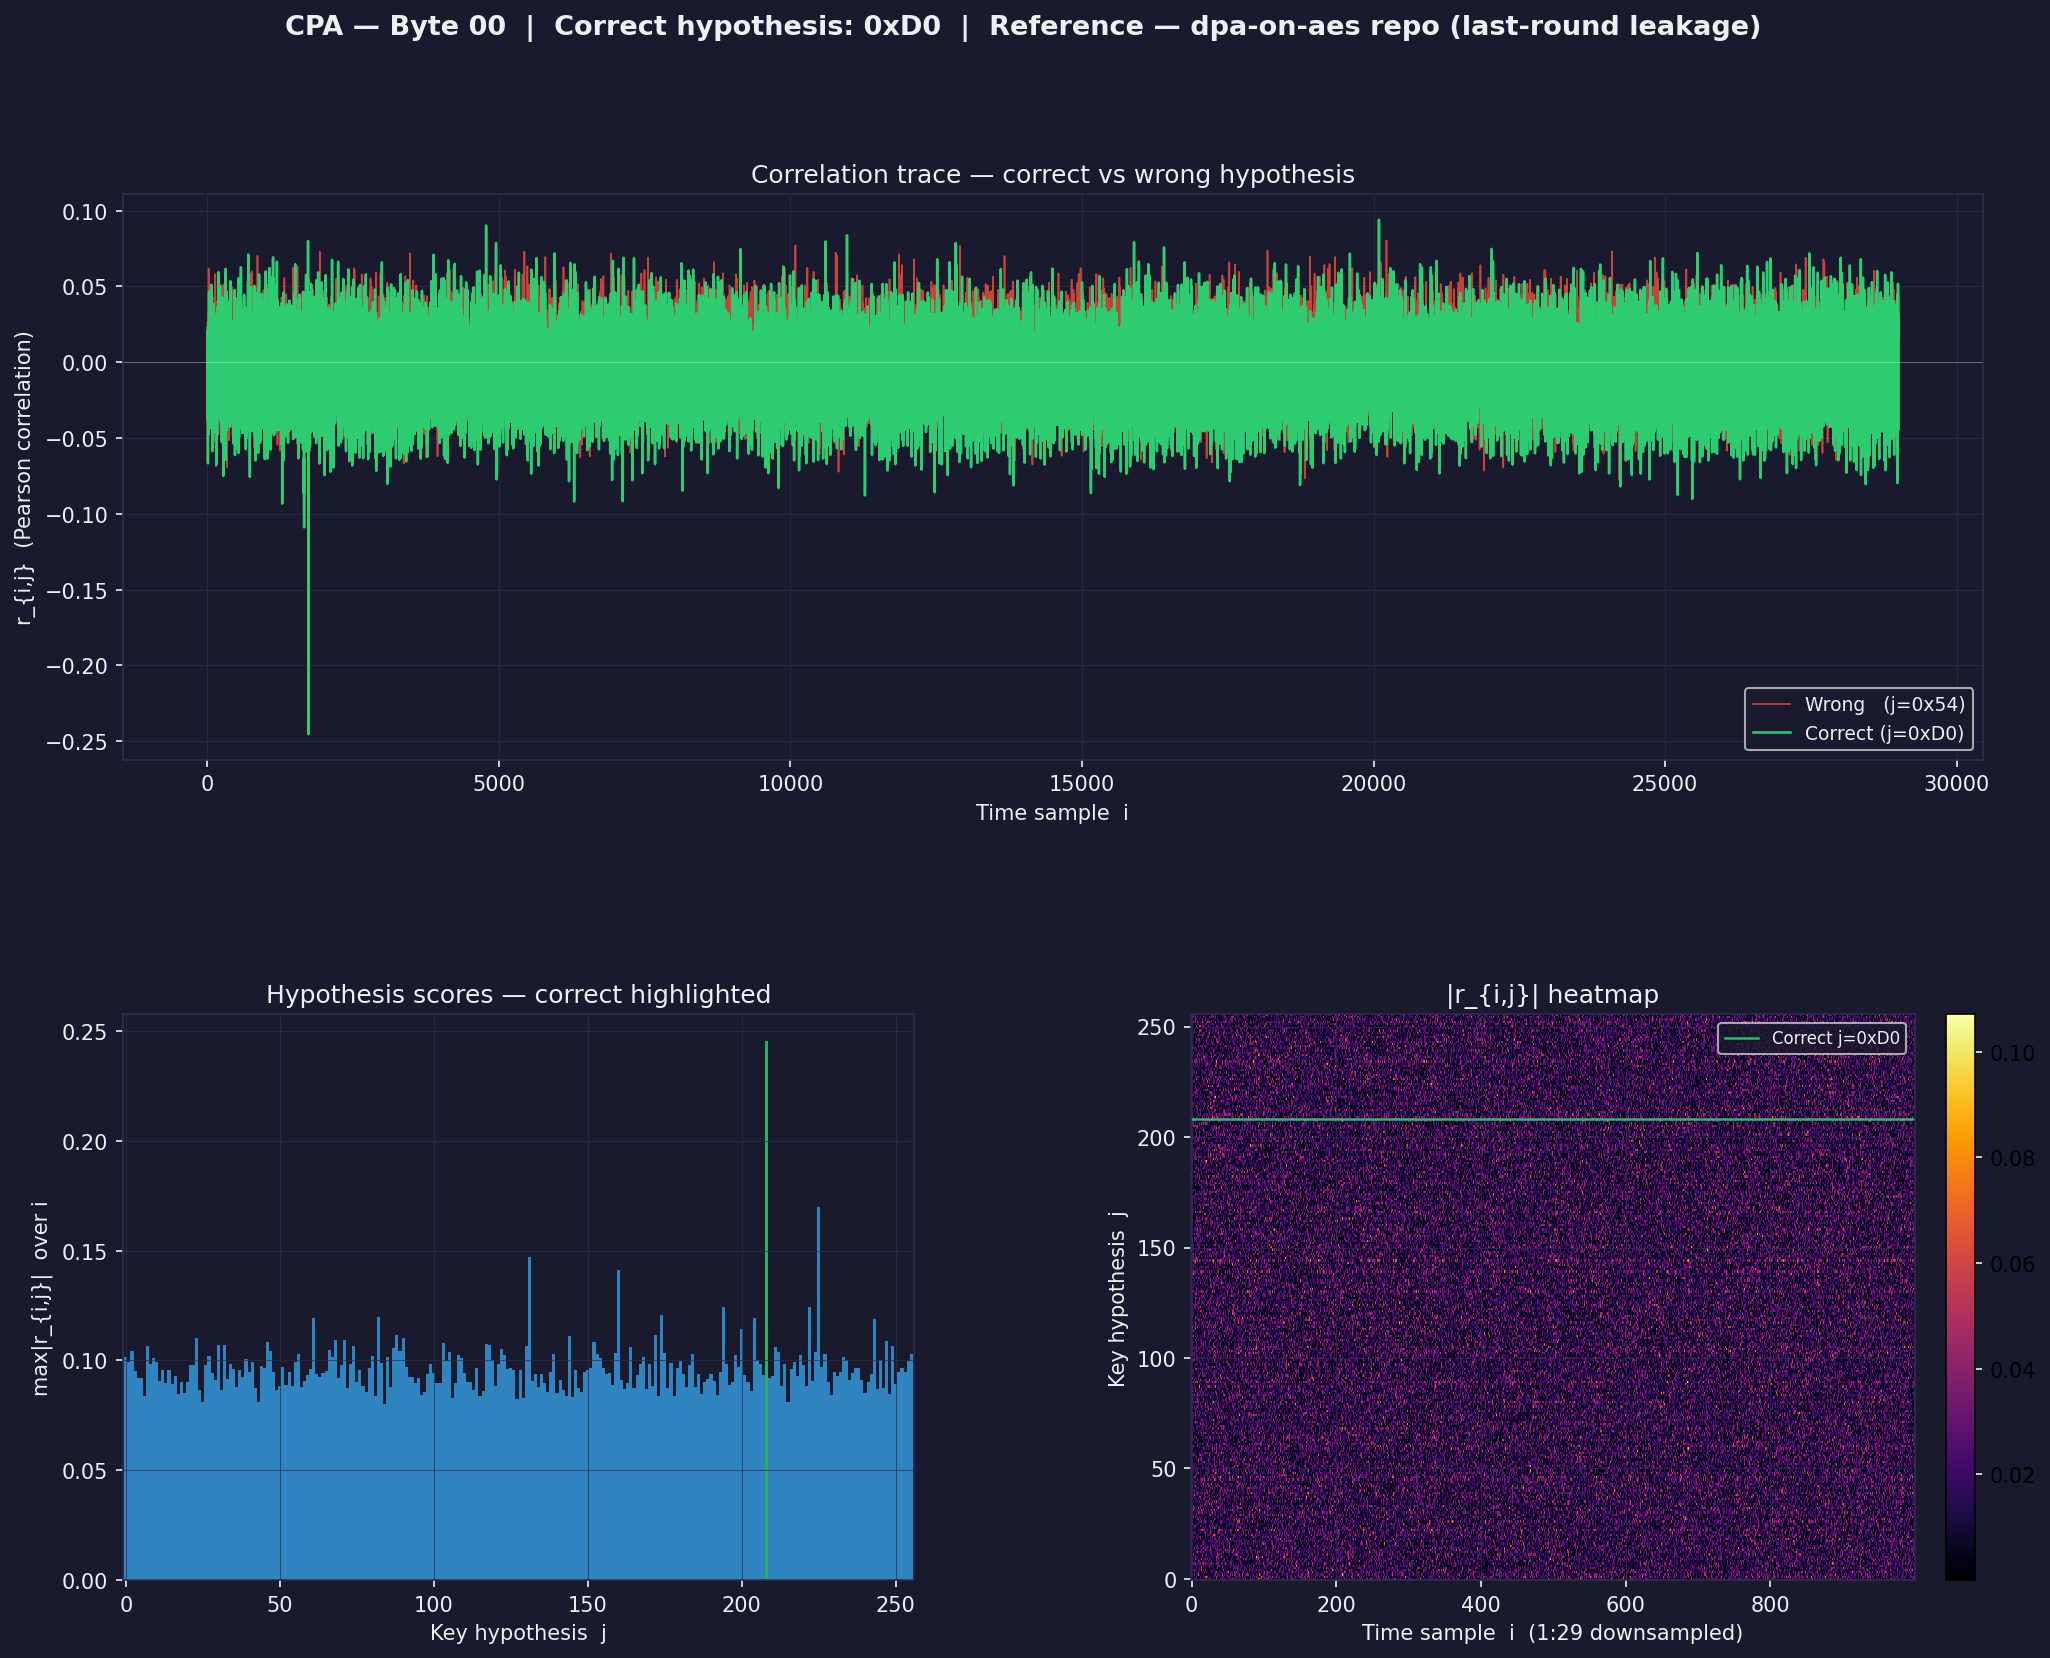
\includegraphics[width=\linewidth]{figures/cpa_byte00.png}
  \caption{CPA diagnostic for key byte 0, $c=2$.
           \textbf{Top}: correlation $r_{i,j}$ over all 29{,}000 time samples
           for the correct hypothesis (green, $j=\texttt{0xD0}$) vs. a wrong
           one (red, $j=\texttt{0x54}$, lowest-scoring).
           The correct guess shows a pronounced negative spike near sample
           1{,}000, corresponding to the last-round SubBytes operation.
           \textbf{Bottom-left}: max $|r_{i,j}|$ across all time samples for
           each of the 256 hypotheses; correct hypothesis (green bar)
           stands clearly above the noise floor.
           \textbf{Bottom-right}: $|r_{i,j}|$ heatmap; the correct
           hypothesis row is the brightest band.}
  \label{fig:cpa}
\end{figure}

\subsection{DPA Key Recovery}

DPA was run with bit position $\ell$ swept from 0 to 7.
Full key recovery was achieved at $\ell = 1$.

\begin{itemize}
  \item \textbf{Bit 0}: 14/16 bytes correct; bytes 3 and 15 wrong.
        Backward key schedule fails verification.
  \item \textbf{Bit 1}: 16/16 bytes correct.
        Recovered round-10 key:
        \texttt{D0 14 F9 A8 C9 EE 25 89 E1 3F 0C C8 B6 63 0C A6}.
        Original key: \texttt{2B 7E 15 16 28 AE D2 A6 AB F7 15 88 09 CF 4F 3C}.
\end{itemize}

Figure~\ref{fig:dpa} shows the DPA diagnostic for byte 0, bit $\ell = 1$.

\begin{figure}[H]
  \centering
  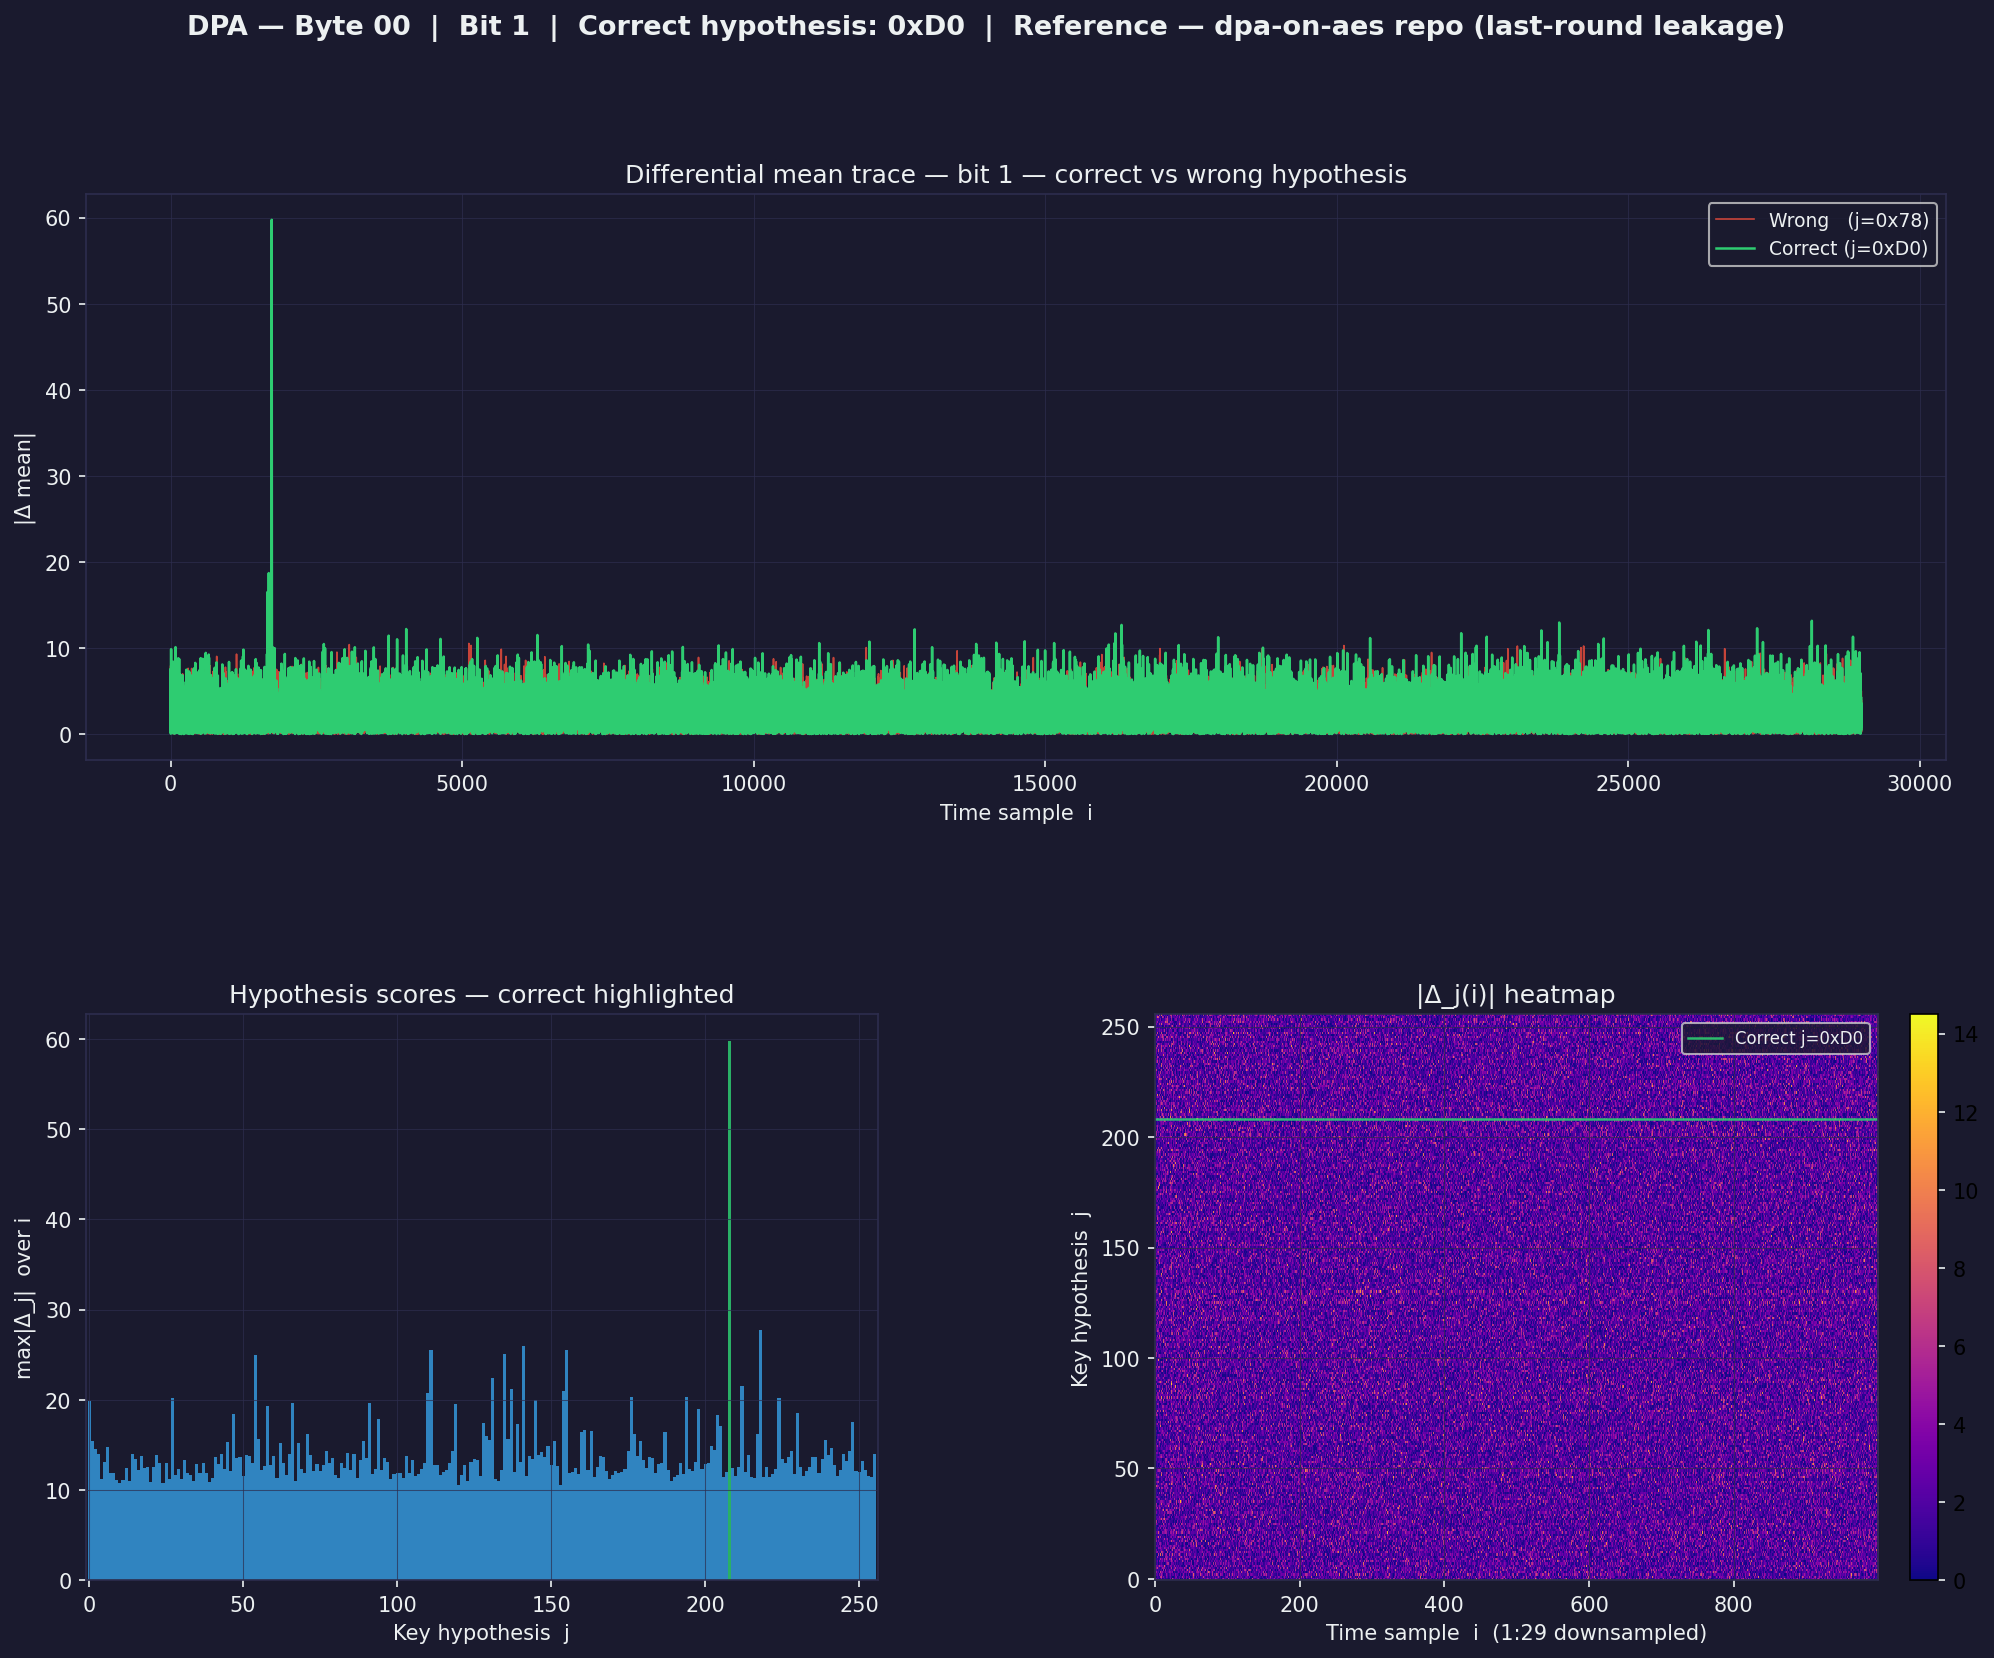
\includegraphics[width=\linewidth]{figures/dpa_byte00_bit1.png}
  \caption{DPA diagnostic for key byte 0, bit $\ell = 1$.
           \textbf{Top}: differential mean $\Delta_j(i)$ over 29{,}000 time
           samples; the correct hypothesis (green, $j=\texttt{0xD0}$) shows a
           sharp peak near the last-round SubBytes window while the wrong
           hypothesis (red) is flat.
           \textbf{Bottom-left}: distinguisher scores for all 256 hypotheses.
           \textbf{Bottom-right}: full $\Delta_j(i)$ heatmap.}
  \label{fig:dpa}
\end{figure}

\subsection{Guessing Entropy}
\label{sec:results:ge}

% ── TODO ──────────────────────────────────────────────────────────────────────
% GE curves require running attacks/guessing_entropy.py on a trace set.
% Once real hardware traces (set_001_pico_real) are collected, replace this
% placeholder with the actual GE vs N_traces plots.
% ─────────────────────────────────────────────────────────────────────────────

\textbf{Note:} Guessing Entropy curves comparing DPA and CPA as a function of
trace count $N$ are pending real hardware trace acquisition
(dataset \texttt{set\_001\_pico\_real}).
The script \texttt{attacks/guessing\_entropy.py} automates GE estimation via
random subsampling trials and will populate this section once traces are
collected.
A placeholder figure location is reserved here for the final submission.

\begin{figure}[H]
  \centering
  \fbox{\parbox{0.9\linewidth}{\centering\vspace{2cm}
    \textit{[PLACEHOLDER]} \\
    GE vs.\ $N_\text{traces}$ for CPA and DPA on \texttt{set\_001\_pico\_real}. \\
    Generated by \texttt{attacks/guessing\_entropy.py --data data/set\_001\_pico\_real}
    \vspace{2cm}}}
  \caption{Guessing Entropy comparison: DPA vs.\ CPA on real Pico hardware
           traces. Target: key byte 0. Horizontal dashed line at GE\,=\,1
           marks full convergence.}
  \label{fig:ge}
\end{figure}

\section{Discussion}
\label{sec:discussion}

\subsection{CPA vs.\ DPA: Efficiency}

Both attacks recover the full 128-bit AES key from 2{,}000 traces on the
reference dataset.
However, the two attacks differ in the structure of their sweep:

\begin{itemize}
  \item \textbf{CPA} requires a sweep of the leakage constant $c$
        (0--255) to handle the HD leakage of byte 11.
        The HW model ($c=0$) already gives rank~1 for 15/16 bytes,
        and $c=2$ resolves the remaining byte.
        The Pearson correlation distinguisher is strictly more data-efficient
        than DPA because it uses the \emph{magnitude} of the hypothetical
        power (not just a single bit), exploiting more signal per trace.

  \item \textbf{DPA} requires a bit-position sweep ($\ell = 0$--7).
        Bit 1 of the last-round intermediate produces clean partitioning for
        all 16 bytes simultaneously.
        DPA is conceptually simpler and makes no assumption about the leakage
        model beyond a single bit's influence on power.
\end{itemize}

\subsection{Byte 11: Hamming Distance Leakage}

The most notable finding is that byte 11 of the round-10 key does not follow
a pure HW leakage model.
Under $c=0$, the CPA score places the correct hypothesis at rank 2
rather than rank 1; $c=2$ (equivalent to $\mathrm{HW}(v \oplus 2)$) resolves
this.
This indicates that the power consumed during the byte-11 operation is
proportional to the number of bit transitions \emph{from state 2} to the
computed intermediate value---a typical HD leakage pattern caused by register
pipeline state.
DPA is unaffected by this because it uses a single bit of $v$ as the
distinguisher, not its full value.

\subsection{Relationship to the AES S-Box Structure}

The attack targets the SubBytes operation because the S-Box is the only
non-linear component in AES.
This is where plaintext (or ciphertext) and key bytes are combined in a way
that is both \emph{computable from known data} (once a key hypothesis is
fixed) and \emph{physically observable} (the S-Box lookup causes data-
dependent switching).
Linear operations (ShiftRows, MixColumns, AddRoundKey) still leak, but their
leakage is linearly predictable from the SubBytes output and thus not
independently useful.

\subsection{Limitations and Open Questions}

\begin{enumerate}
  \item \textbf{Real hardware GE curves.}
    The reference dataset traces have $T = 29{,}000$ samples; the Pico
    acquisition is configured for $T = 5{,}000$ samples.
    The GE analysis (Section~\ref{sec:results:ge}) on real Pico traces
    is the primary pending deliverable.

  \item \textbf{Masking countermeasure.}
    The current firmware has no countermeasures.
    Applying first-order Boolean masking to the S-Box lookup would break
    first-order CPA/DPA and requires a second-order attack.
    This is a natural extension.

  \item \textbf{Alignment sensitivity.}
    Traces must be aligned on the trigger edge for both attacks to function.
    Even a one-sample misalignment spreads the leakage signal across adjacent
    samples and reduces distinguisher scores.
    The hardware trigger (GPIO\,22) provides sample-accurate alignment for
    this setup.
\end{enumerate}

\section{Conclusion and Future Work}
\label{sec:conclusion}

\subsection{Summary}

This project implemented and evaluated two classical power side-channel attacks
---DPA and CPA---targeting AES-128 on an RP2040 microcontroller.

\begin{itemize}
  \item A complete hardware test bench was built: Pico firmware with a hardware
        trigger, pyvisa-based oscilloscope acquisition, and a structured
        \texttt{.npy} dataset format.

  \item CPA with the Pearson correlation distinguisher recovers all 16 bytes
        of the round-10 key at rank 1 using 2{,}000 traces.
        Fifteen bytes succeed under the HW model ($c=0$); byte 11 requires
        an HD model ($c=2$).

  \item DPA with the differential-mean distinguisher recovers all 16 bytes
        at bit position $\ell=1$ using the same 2{,}000 traces.

  \item Both attacks recover the original 128-bit key
        (\texttt{2B 7E 15 16 28 AE D2 A6 AB F7 15 88 09 CF 4F 3C})
        via backward key schedule.

  \item The byte-11 HD leakage finding provides a concrete example of
        how leakage model selection affects CPA but not DPA, highlighting a
        practical advantage of DPA in model-agnostic scenarios.
\end{itemize}

\subsection{Future Work}

\begin{description}
  \item[Guessing Entropy on real hardware traces.]
    Once acquisition on the physical Pico is complete
    (\texttt{attacks/guessing\_entropy.py --data data/set\_001\_pico\_real}),
    GE vs.\ $N_\text{traces}$ curves for both attacks will provide a
    quantitative trace-complexity comparison.

  \item[Masking countermeasure evaluation.]
    Applying Boolean masking (first-order) to the firmware S-Box lookup
    and measuring the increase in required traces for second-order attacks
    would directly address the defense portion of the proposal.

  \item[SNR characterisation across noise levels.]
    Injecting controlled additive noise into simulated traces and measuring
    at what SNR each attack fails would produce the characterisation proposed
    in the original plan.

  \item[EM side channel.]
    Replacing the power probe with an EM probe positioned over the RP2040
    core would allow comparison of power vs.\ EM leakage on the same target.
\end{description}


% ── References ────────────────────────────────────────────────────────────────
\bibliographystyle{ieeetr}
\bibliography{references}

% ── Appendices ────────────────────────────────────────────────────────────────
\appendix
\section{Hardware Setup and Oscilloscope Capture}
\label{app:hw}

\subsection{Board Comparison}

\begin{table}[H]
\centering
\caption{All boards evaluated in this project.}
\begin{tabular}{@{}p{4.2cm}p{3.5cm}p{2.3cm}p{4cm}@{}}
\toprule
Board & MCU & Outcome & Root cause \\
\midrule
Raspberry Pi Pico & RP2040, Cortex-M0+, 125\,MHz & Failed &
  On-chip SMPS ($\approx$1\,MHz switching noise on DVDD) \\
Arduino Uno R4 Minima & Renesas RA4M1, Cortex-M4, 48\,MHz & Failed &
  Internal DC-DC regulation + only 2{,}000 traces \\
\textbf{Adafruit Pro Tinkrer 5\,V} & \textbf{ATmega328P, 16\,MHz} &
  \textbf{Success} & Clean 5\,V linear supply; no SMPS \\
\bottomrule
\end{tabular}
\end{table}

\subsection{Pro Tinkrer 5\,V @ 16\,MHz Setup}
\label{app:hw:trinket}

\textbf{Target:} Adafruit Pro Tinkrer 5\,V 16\,MHz~\cite{adafruit_trinket_pro}
(ATmega328P~\cite{atmega328p}, same MCU as the classic Arduino Uno).

\subsubsection*{Wiring Diagram}

\begin{verbatim}
USB 5V ----+---- [10 Ohm shunt] ----+---- Pro Tinkrer VCC pin
           |                        |
           |              [scope CH1+]  <- Keysight oscilloscope (differential)
           |              [scope CH1-] -- GND
           |
           +-- GND -------------------------------- Trinket GND pin

Trigger:
  Trinket GPIO 8 ----------- scope CH2 / EXT TRIG BNC (rising edge)

Host serial:
  USB-UART adapter (FTDI) -- /dev/tty.usbserial-XXXX
  Trinket TX/RX ------------ adapter RX/TX
  Baud: 115200
\end{verbatim}

% TODO-SCHEMATIC-FIGURE: Replace the text diagram above with a proper figure.
% Suggested path: report/figures/trinket_schematic.png
% Uncomment and fill in once the image is ready:
%
% \begin{figure}[H]
%   \centering
%   \includegraphics[width=0.85\linewidth]{figures/trinket_schematic.png}
%   \caption{Pro Tinkrer 5\,V measurement setup schematic. 10\,$\Omega$
%            shunt on VCC rail; GPIO\,15 trigger to scope CH2.}
%   \label{fig:schematic}
% \end{figure}

\subsubsection*{Oscilloscope Settings}

\begin{itemize}
  \item \textbf{Model:} Keysight / Agilent oscilloscope\\
        VISA address: \texttt{USB0::0x2A8D::0x17B6::MY65060127::INSTR}
  \item \textbf{Backend:} PyVISA-py (USBTMC, no proprietary driver required)
  \item \textbf{Channel 1:} power trace (differential across 10\,$\Omega$ shunt)
  \item \textbf{Channel 2 / EXT:} hardware trigger (GPIO\,8 rising edge)
  \item \textbf{Trigger:} rising edge, CH2; \textbf{single-shot} mode
  \item \textbf{Sample rate:} $\geq$\,250\,MS/s
  \item \textbf{Points per acquisition:} 30{,}000 (BYTE format, uint8 ADC counts)
\end{itemize}

Key SCPI commands used:
\begin{verbatim}
:WAVeform:SOURce CHANnel1    -- power trace from CH1
:WAVeform:FORMat BYTE        -- binary uint8 transfer
:WAVeform:POINts:MODE NORMal
:WAVeform:POINts 30000       -- 30k samples per trigger
:SINGle                      -- arm single-shot trigger
*OPC?                        -- wait for acquisition complete
:WAVeform:DATA?              -- download waveform
\end{verbatim}

\subsubsection*{Capture Command (50k traces)}

\begin{verbatim}
python capture/capture.py \
  --board adafruit_trinket_pro_5v16mhz \
  --port /dev/tty.usbmodem101 \
  --num-traces 50000 \
  --baud 115200 \
  --serial-delay 0.5 \
  --scope-address USB0::0x2A8D::0x17B6::MY65060127::INSTR \
  --scope-channel CHANnel1 \
  --scope-points 30000 \
  --notes "shunt on 5V VCC, 10 Ohm"
\end{verbatim}

% TODO-TRINKET-CAPTURE: Run the command above to capture 50,000 traces.
% Output: data/set_004_trinket_*/traces.npy, plaintexts.npy, ciphertexts.npy

\subsection{Circuit Photographs}
\label{app:hw:photos}

\begin{figure}[H]
  \centering
  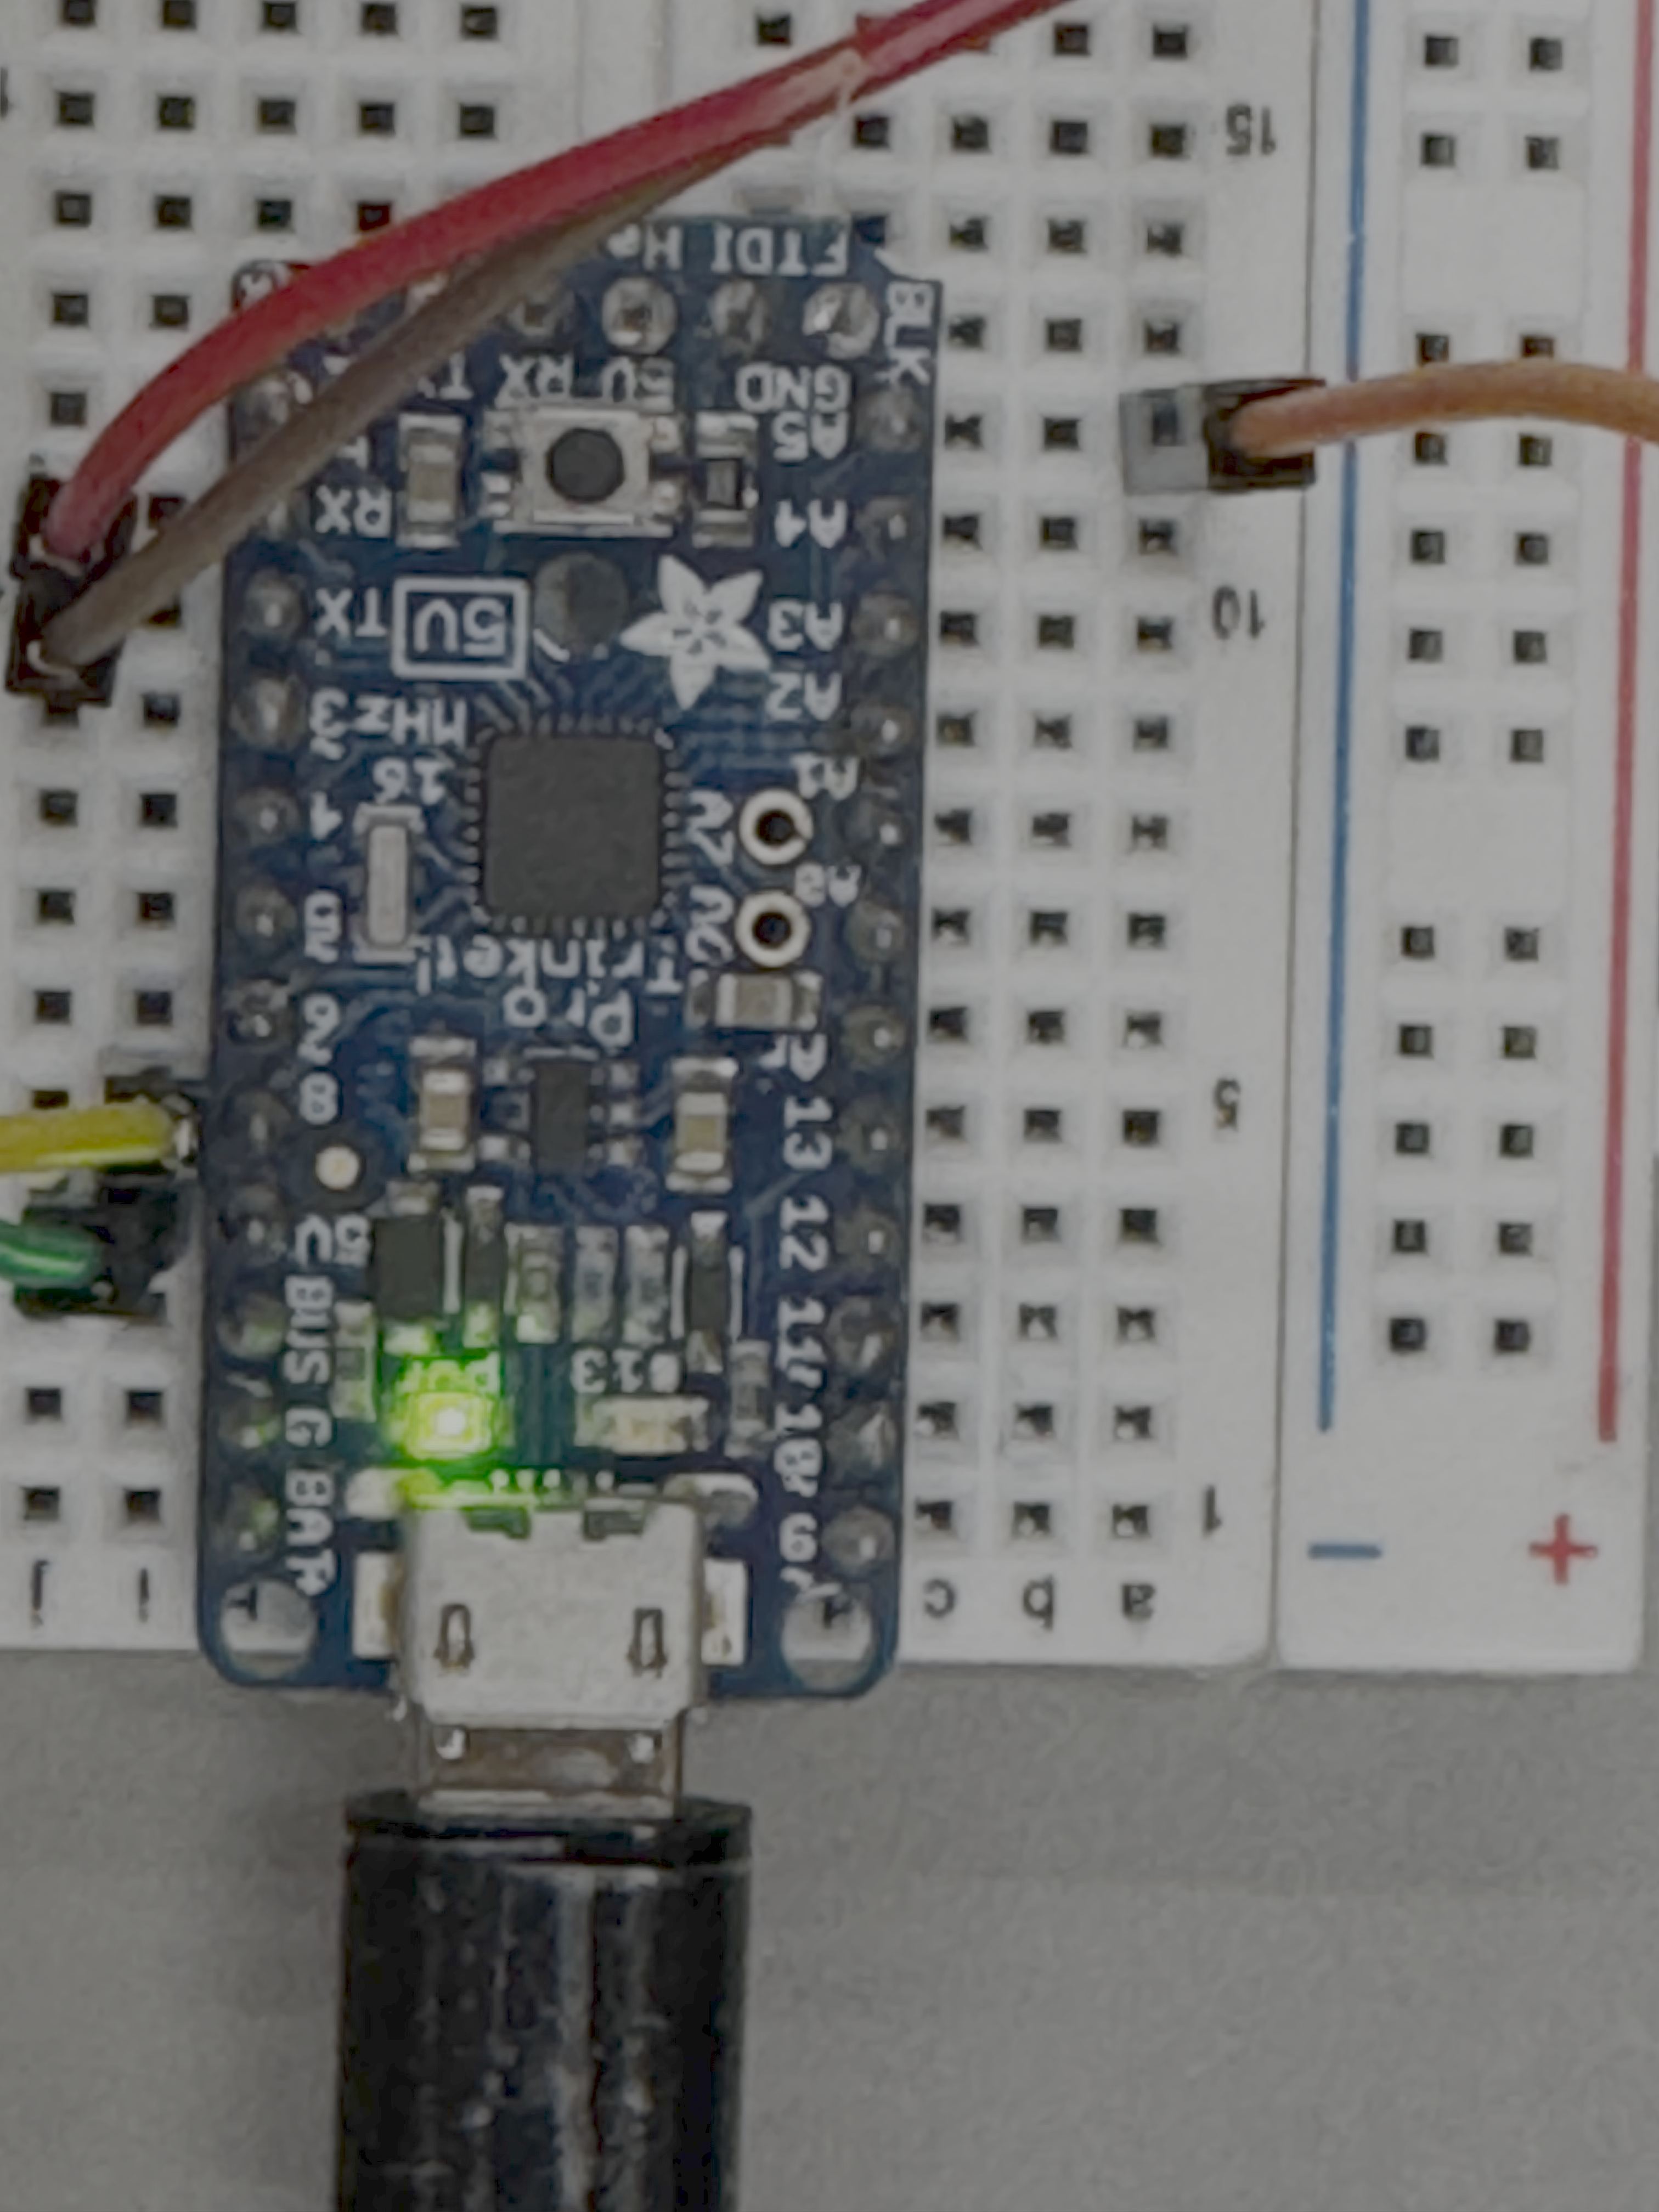
\includegraphics[width=0.85\linewidth]{figures/experiment_hw/board_setup_adfruit_tinkrer_v16mhz_circuit_used_to_attack.png}
  \caption{Pro Tinkrer 5\,V close-up bench setup used for all SCA captures.
           The 10\,$\Omega$ shunt is placed in series with the VCC rail;
           oscilloscope CH1 (differential) measures the voltage drop across
           the shunt proportional to processor current.
           GPIO\,8 is wired to scope CH2 as the hardware trigger.
           The FTDI USB-UART adapter (right) provides the serial plaintext
           channel at 115200\,baud.}
  \label{fig:circuit_trinket}
\end{figure}

\begin{figure}[H]
  \centering
  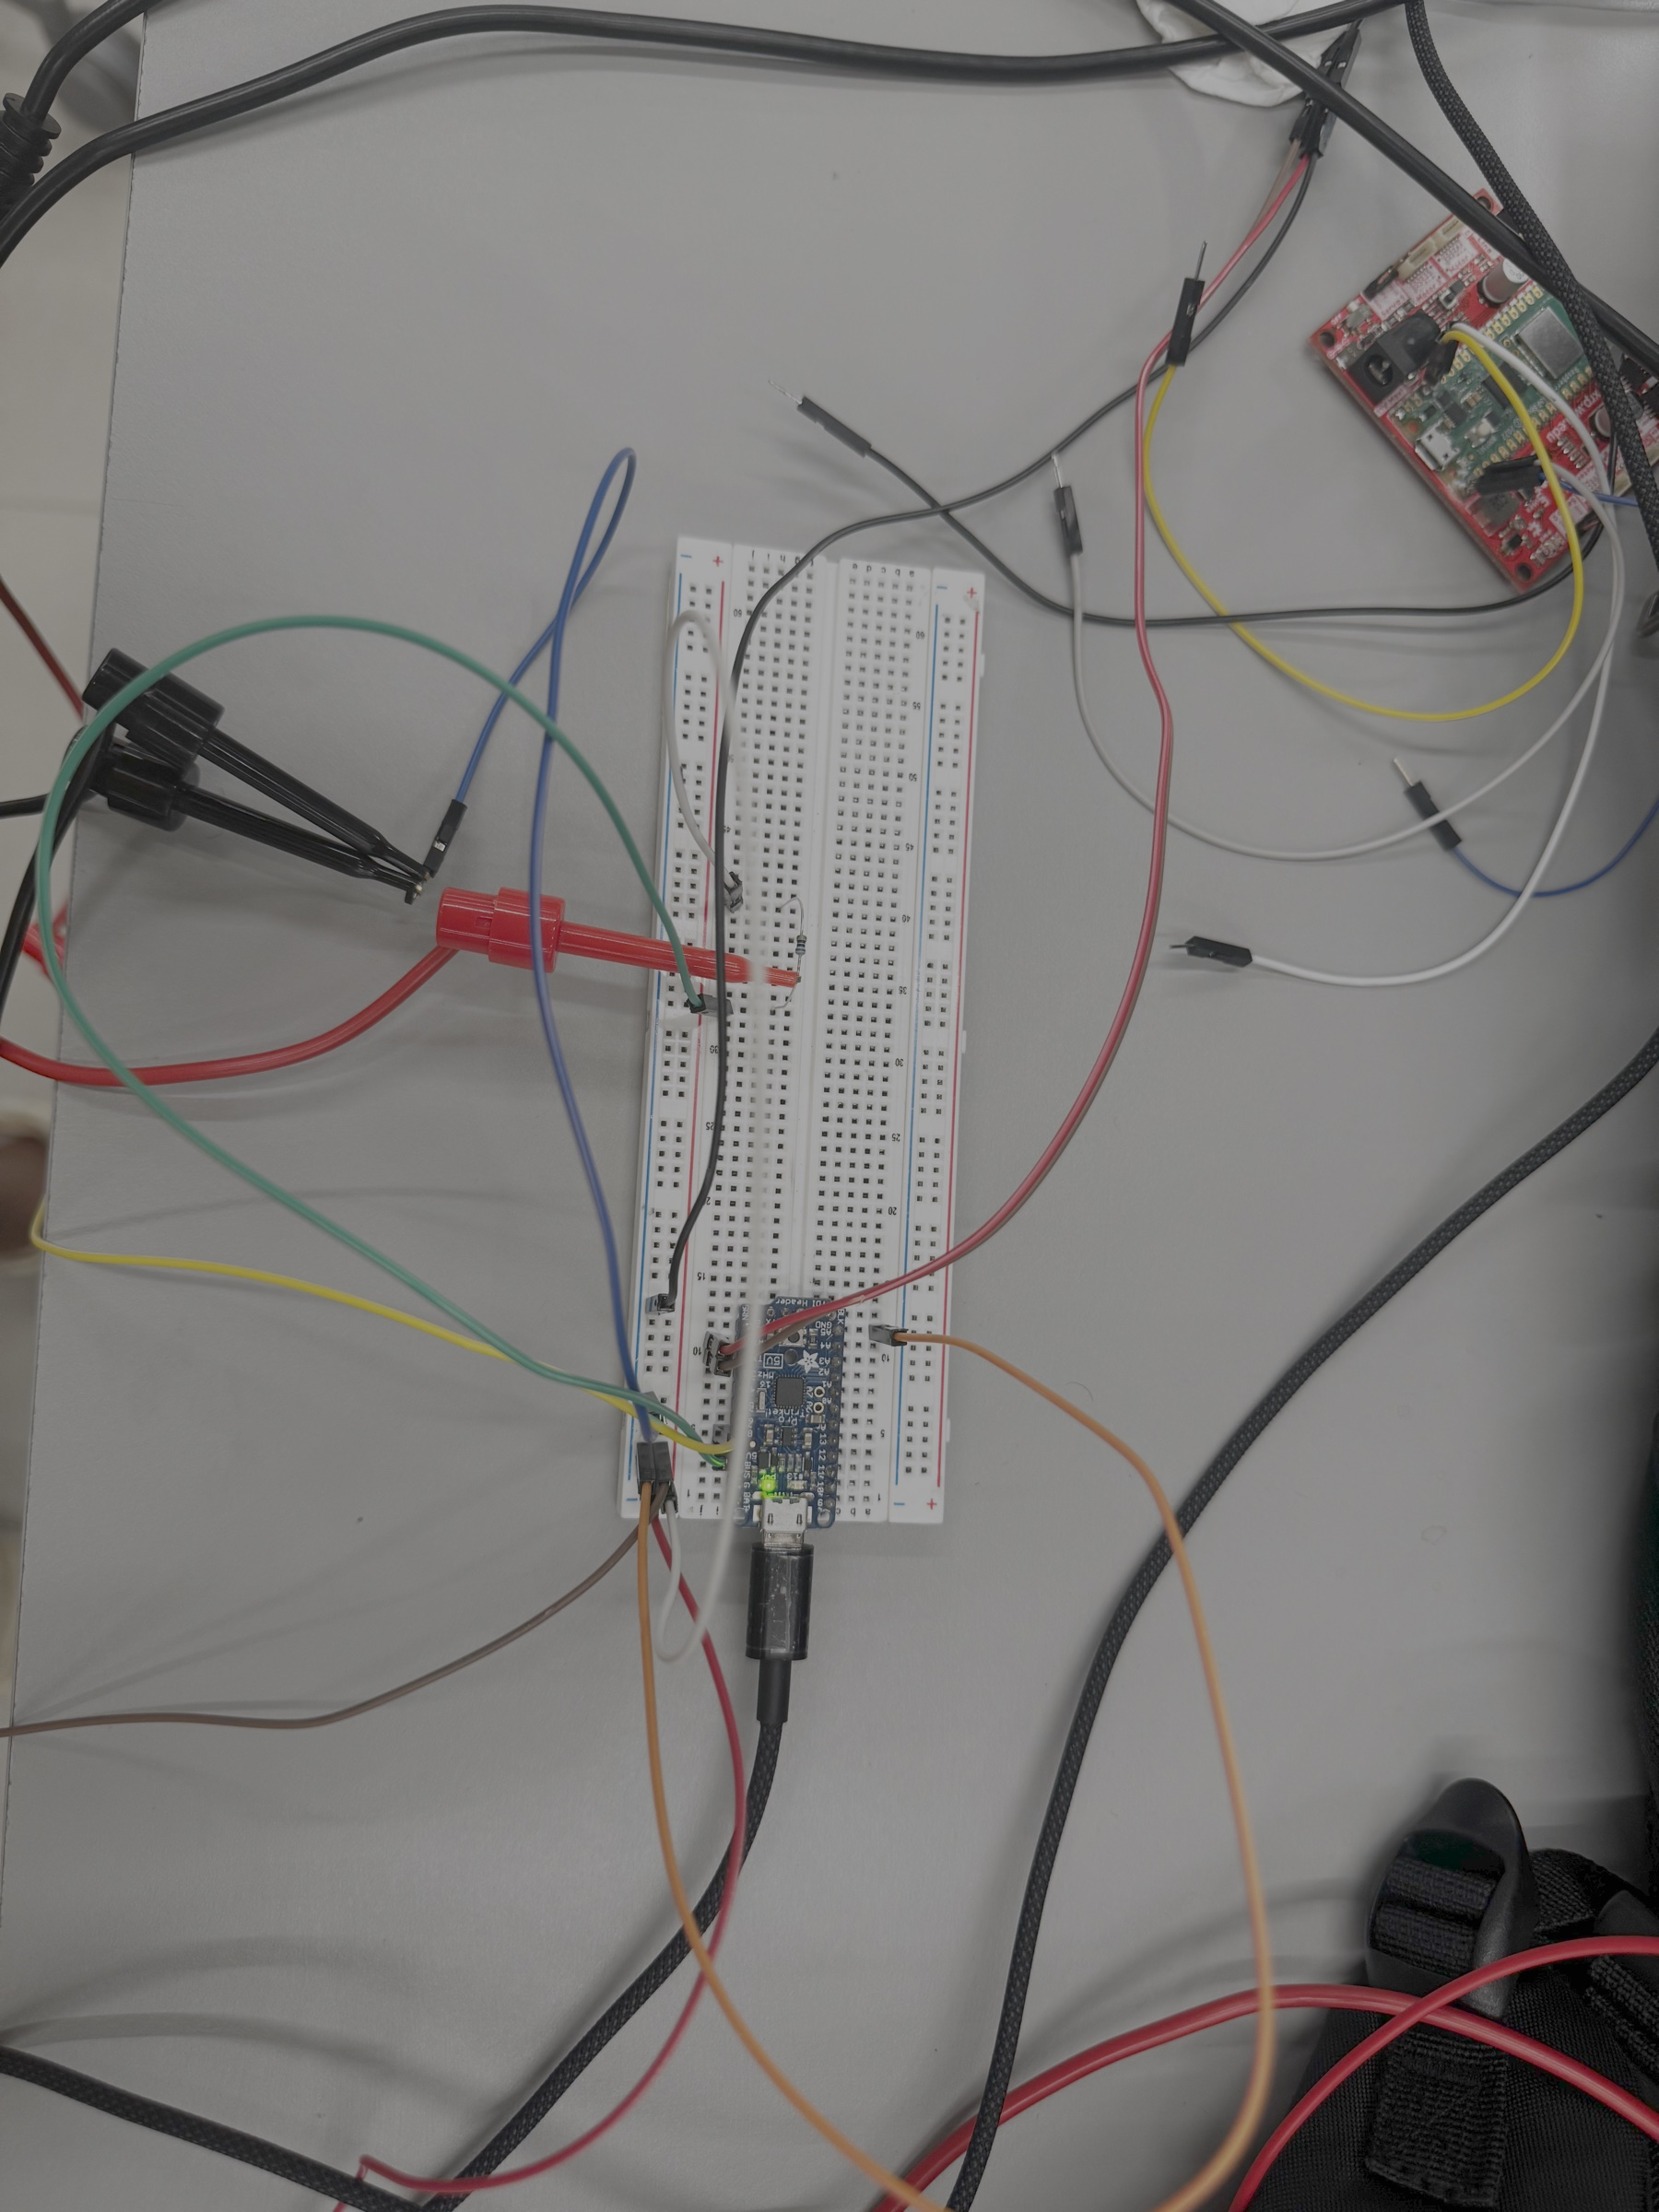
\includegraphics[width=0.85\linewidth]{figures/experiment_hw/full_circuit_picture_detkin_lab.jpg}
  \caption{Full lab bench setup in Detkin Lab.
           Left: Keysight oscilloscope displaying the AES-128 power trace
           on CH1 (differential across 10\,$\Omega$ shunt on VCC rail) and
           the GPIO\,8 hardware trigger on CH2.
           Right: Pro Tinkrer 5\,V with shunt and FTDI USB-UART adapter
           connected to the host capture script.}
  \label{fig:circuit_full}
\end{figure}

% TODO-CIRCUIT-PICO: Insert a photograph of the RPi Pico bench setup.
% Place at report/figures/circuit_pico.jpg and uncomment:
%
% \begin{figure}[H]
%   \centering
%   \includegraphics[width=0.85\linewidth]{figures/circuit_pico.jpg}
%   \caption{RPi Pico RP2040 measurement setup.
%            Shunt placed on GND rail; trigger on GPIO\,22.
%            Attack did not converge due to on-chip SMPS noise
%            (Section~\ref{sec:discussion:hw}).}
%   \label{fig:circuit_pico}
% \end{figure}

\subsection{Video and Photographic Evidence}
\label{app:hw:video}

Video recordings and photographic evidence of the oscilloscope capture
session are hosted in the project repository.
All media links are consolidated in the \textbf{README} under
\emph{Hardware Setup $\to$ Video Demos}:

\begin{center}
  \url{https://github.com/navjotschahal/power_analysis_sca}
\end{center}

The recordings document:

\begin{itemize}
  \item \textbf{Oscilloscope trigger:} GPIO\,8 rising edge firing on the
        Pro Tinkrer , visible on scope CH2.
  \item \textbf{AES power trace:} the first-round AES-128 computation visible
        as elevated switching activity on scope CH1 (differential across
        10\,$\Omega$ shunt).
  \item \textbf{Capture script:} Python acquisition running in terminal with
        \texttt{tqdm} progress bar and per-trace serial latency output.
  \item \textbf{Circuit bench:} Pro Tinkrer with shunt, FTDI adapter, and
        Keysight oscilloscope connections.
\end{itemize}

\noindent
The dataset itself (traces, plaintexts, ciphertexts) is available for
download from Google Drive (link in README):

\begin{center}
  \href{https://drive.google.com/file/d/1Itl82UCQEDyk6cYDD33kB-gKtlXIQBZe/view?usp=sharing}%
       {Google Drive --- Power Trace Dataset (Pro Tinkrer 5\,V, 30{,}000 samples/trace)}
\end{center}

\section{Software Repository}
\label{app:repo}

The full source code, capture scripts, attack implementations, and
documentation are available at:

\begin{center}
  \url{https://github.com/navjotschahal/power_analysis_sca}
\end{center}

\subsection*{Project Deliverables}

\begin{description}
  \item[Project Proposal]
    The initial project proposal is available in the repository root:\\
    \href{https://github.com/navjotschahal/power_analysis_sca/blob/main/nschahal_proposal-1.pdf}%
         {\texttt{nschahal\_proposal-1.pdf}}
    (see \texttt{README.md} for direct link).

  \item[Project Presentation]
    The slide deck is linked from the repository README under
    \emph{Project Deliverables $\to$ Presentation}:\\
    \url{https://github.com/navjotschahal/power_analysis_sca}

  \item[Experiment Media (Videos \& Photos)]
    All lab videos (oscilloscope capture session, trigger firing,
    AES power trace, acquisition script) and circuit bench photographs
    are linked in the repository README under
    \emph{Hardware Setup $\to$ Video Demos}:\\
    \url{https://github.com/navjotschahal/power_analysis_sca}

  \item[Dataset Download]
    Captured power traces (Pro Tinkrer 5\,V, up to 30{,}000 samples/trace)
    are hosted on Google Drive (link in README):\\
    \href{https://drive.google.com/file/d/1Itl82UCQEDyk6cYDD33kB-gKtlXIQBZe/view?usp=sharing}%
         {Google Drive --- Power Trace Dataset}
\end{description}

\subsection{Repository Structure}

\begin{verbatim}
power_analysis_sca/
  README.md
  firmware/
    main.cpp              AES-128 firmware (GPIO trigger, tiny-AES-c)
    CMakeLists.txt        AVR/Pico SDK CMake build
  capture/
    capture.py            Unified pyvisa + pyserial acquisition (all boards)
    examples.txt          Example capture commands per board
  data/
    DATA_FORMAT.md        Schema: shapes, dtypes, row alignment
    set_001_pico_real/    RPi Pico traces (100 traces, did not converge)
    set_002_reference/    ChipWhisperer reference (2000x29000, working)
      traces.npy          (2000, 29000) float32
      plaintexts.npy      (2000, 16)   uint8
      ciphertexts.npy     (2000, 16)   uint8
      meta.json           key, attack_round=last, label
      plots/              Generated diagnostic figures
    set_003_arduino_shuntGND/  Arduino Uno R4 (2000 traces, did not converge)
    set_004_trinket_*/    Pro Tinkrer 5V (50k traces planned)
  attacks/
    helper.py             Shared AES tables, key schedule, load_dataset
    classical/
      cpa.py              CPA: Pearson correlation, const sweep 0-255
      dpa.py              DPA: differential mean, bit sweep 0-7
      guessing_entropy.py GE(N) curves, DPA vs CPA comparison
    deep_learning/
      hettwer_sca.py      Hettwer 2020 CNN -- train + KGE evaluation
      image_encode.py     GASF / GADF / RP / MTF encoders
      device.py           GPU/CPU device detection helper
  references/
    dpa-on-aes/           Cloned reference notebook (original .txt traces)
  report/                 This LaTeX report
    main.tex
    references.bib
    sections/             One .tex per section
    appendix/             One .tex per appendix
    figures/              PNG figures for includegraphics
\end{verbatim}

\subsection{Reproducing All Results}

\begin{enumerate}
  \item \textbf{Run CPA on reference dataset}
\begin{verbatim}
python attacks/classical/cpa.py \
  --data data/set_002_reference --round last
\end{verbatim}
  Output: \texttt{data/set\_002\_reference/plots/cpa\_byte00.png}
  (and one plot per byte).

  \item \textbf{Run DPA on reference dataset}
\begin{verbatim}
python attacks/classical/dpa.py \
  --data data/set_002_reference --round last
\end{verbatim}
  Output: \texttt{data/set\_002\_reference/plots/dpa\_byte00\_bit1.png}.

  \item \textbf{Generate Guessing Entropy curves}
\begin{verbatim}
python attacks/classical/guessing_entropy.py \
  --data data/set_002_reference --byte 0 --trials 20 --steps 20
\end{verbatim}
  Output: \texttt{data/set\_002\_reference/plots/ge\_comparison\_b00.png}.

  \item \textbf{Visualise image encoding pipeline}
\begin{verbatim}
python attacks/deep_learning/image_encode.py \
  --data data/set_002_reference --show
\end{verbatim}
  Output: \texttt{data/set\_002\_reference/plots/image\_encoding\_gallery\_b00.png}.

  \item \textbf{Train Hettwer CNN and evaluate KGE}
\begin{verbatim}
python attacks/deep_learning/hettwer_sca.py \
  --data data/set_002_reference --round last \
  --channels gasf+gadf --byte 0
\end{verbatim}
  Outputs: \texttt{hettwer\_gasf+gadf\_training\_b00.png},
           \texttt{hettwer\_gasf+gadf\_ge\_b00.png}.

  \item \textbf{Capture real traces from Pro Tinkrer } (hardware required)
\begin{verbatim}
python capture/capture.py \
  --board adafruit_trinket_pro_5v16mhz \
  --port /dev/tty.usbmodem101 \
  --num-traces 50000 --scope-points 30000
\end{verbatim}
\end{enumerate}

\noindent
All scripts read dataset path, attack parameters, and known key from
\texttt{meta.json}; no hardcoded paths.
Generated plots are saved to \texttt{data/<set>/plots/}.


\end{document}
